\begin{frame}
  \frametitle{What is a Compiler?}

    \onslide<1->{
  \begin{block}{Basically}
    A compiler is a language translator. It translates from one programming language to another. (E.g. C to Assembly, Java to C, C++ to C)
  \end{block}
  }

    \onslide<2->{
  \begin{block}{We can say...}
    A compiler processes \textit{programming language}. Or in other words, a compiler is a kind of \textit{language} processor.
  \end{block}
  }

\end{frame}

\begin{frame}
  \frametitle{Human translators behave like a Compiler}

\begin{pspicture}(0,0)(124,140) % without grid
    %\psframe(0,0)(62,70)

    \putnode{n1}{origin}{20}{30}{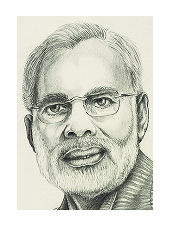
\includegraphics[natwidth=66,natheight=93,width=66pt]{images/modi.eps}}

    \putnode{n2}{origin}{200}{30}{
\includegraphics[natwidth=236,natheight=308,width=66pt]{images/trump.eps}}

    \putnode{n22}{n1}{0}{55}{}
    \putnode{n23}{n2}{0}{55}{}


    \only<2->{\putnode{n3}{origin}{110}{100}{
\includegraphics[natwidth=116,natheight=139,width=66pt]{images/woman.eps}}}

    \only<2->{\putnode{n21}{n3}{-25}{0}{}
    \putnode{n24}{n3}{25}{0}{}}

    \only<1>{\putnode{n7}{origin}{75}{100}{\cfgcode{PM Modi wants to speak in Hindi.\newline{} But Mr. Trump doesn't know Hindi.}}}

    \only<3->{\putnode{n8}{n1}{0}{48}{\cfgcode{Aapko jeet ki bohot badhai.}}}
    \only<3->{\putnode{n9}{n1}{10}{41}{\cfgcode{Aasha hai ham milkar kaam karenge.}}}

    \only<4->{\putnode{n8}{n2}{0}{45}{\cfgcode{Congratulations on the win.}}}
    \only<4->{\putnode{n9}{n2}{0}{38}{\cfgcode{We wish to work together.}}}

    \putnode{n4}{n1}{0}{-38}{\cfgcode{PM Modi}}
    \putnode{n5}{n2}{0}{-35}{\cfgcode{POTUS}}
    \only<2->{\putnode{n6}{n3}{0}{-35}{\cfgcode{Translator}}}

    \only<3->{\nccurve[angleA=45,angleB=180,ncurv=1]{->}{n22}{n21}}
    \only<4->{\nccurve[angleA=0,angleB=90,ncurv=1]{->}{n24}{n23}}

    \only<5->{\putnode{n30}{n3}{0}{-60}{\psframebox[fillstyle=solid,fillcolor=lightgray,opacity=0.8]{She is working like a compiler!}}}

    \only<6->{\putnode{n31}{n3}{60}{40}{\psframebox[fillstyle=solid,fillcolor=lightgray,opacity=0.8]{Meaning is preserved!!}}}
\end{pspicture}


\end{frame}


\begin{frame}
  \frametitle{Compiler}
    \begin{block}{Precisely...}
        Compiler is a software that translates the input language program into a target language program, with equivalent meaning.
    \end{block}
%    \vspace*{\fill}

\begin{pspicture}(0,0)(124,100) % without grid
    %\psframe(0,0)(62,70)
    \putnode{n1}{origin}{110}{70}{\psframebox{\cfgcode{COMPILER}}}

    \putnode{n2}{n1}{-50}{0}{\cfgcode{Source Progarm}}
    \putnode{n21}{n2}{20}{0}{}

    \putnode{n3}{n1}{50}{0}{\cfgcode{Target Program}}
    \putnode{n31}{n3}{-20}{0}{}

    \ncline{->}{n21}{n1}
    \ncline{->}{n1}{n31}

    \only<2->{
    \putnode{n4}{origin}{110}{20}{\psframebox{\cfgcode{INTERPRETER}}}

    \putnode{n5}{n4}{-60}{5}{\cfgcode{Source Progarm}}
    \putnode{n51}{n5}{22}{0}{}

    \putnode{n7}{n4}{-60}{-5}{\cfgcode{Input}}
    \putnode{n71}{n7}{12}{0}{}

    \putnode{n6}{n4}{50}{0}{\cfgcode{Output}}
    \putnode{n61}{n6}{-15}{0}{}

    \ncline{->}{n71}{n4}
    \ncline{->}{n51}{n4}
    \ncline{->}{n4}{n61}
}

\end{pspicture}


\end{frame}


\begin{frame}
  \frametitle{Phases of a Compiler}
    \begin{block}{Compiler is a BIG Algorithm}
        Its is so big that it comprises of hundereds of sub-algorithms. And like any algorithm, Compilers work in a step-by-step fashion. These steps are called phases.
    \end{block}
    \onslide<2->{
    \begin{enumerate}
        \item Lexical Analyzer (covered here)
        \item Syntax Analyzer (partially covered here)
        \item Semantic Analyzer
        \item Intermediate Code Generator
        \item Machine-Independent Optimizer
        \item Target Code Generator
        \item Machine-Dependent Optimizer
    \end{enumerate}
}
\end{frame}


\begin{frame}[fragile]
  \frametitle{Lexical Analysis}
    \begin{block}{}
        Input : \Term{Raw Program}, Output : \Term{Stream of Tokens}
    \end{block}

    \begin{lstlisting}[language=C, frame=leftline,]
int main() { // C program
    int sum;
    sum = 10 + 15 * 6;
}
\end{lstlisting}

    \begin{itemize}
        \item<2-> Lets only consider statement \Codetb{3} for our purpose.
        \item<3-> This program is adding \Codetb{10} with the product of \Codetb{15} and \Codetb{6}, and storing it in an \Codet{int} variable \Code{sum}.
        \item<4-> The smallest logical units on line \Codetb{3} are : \Code{sum}, \Code{=}, \Codetb{10}, \Code{+}, \Codetb{15}, \Code{*}, \Codetb{6} and \Codeb{;}. These are called \textbf{Lexemes}.
        \item<5-> Lexical Analyzer extracts these lexemes and converts them into \textbf{tokens}.
    \end{itemize}
\end{frame}


\begin{frame}
  \frametitle{What are Tokens?}
    \begin{block}{}
        Tokens are generalization of Lexemes.
    \end{block}

    \begin{itemize}
        \item<1-> Tokens provide important information about the lexemes.
        \item<2-> For example, lexeme \Codetb{10} is converted to a token like \texttt{<num, 10>}. Similarly other constants are converted to, \texttt{<num, 15>}, \texttt{<num, 6>}.
        \item<3-> One of the task of Lexical Analyzer is to classify the lexemes. Here, \Codetb{10}, \Codetb{15}, \Code{6} are classified as a number.
        \item<4-> Similarly, \Code{sum} is classified as an \texttt{identifier}. And can be represented as \texttt{<id, sum>}

    \end{itemize}
\end{frame}


\begin{frame}[fragile]
  \frametitle{Input/Output of Lexical Analyzer}
    If input is this line,

    \begin{lstlisting}[language=C, frame=leftline,]
    sum = 10 + 15 * 6;
\end{lstlisting}

    \begin{block}{then lexemes are}
        \DCode{sum} \DCode{=} \DCodetb{10} \DCode{+} \DCodetb{15} \DCode{*} \DCodetb{6} \DCodeb{;}
    \end{block}

    \begin{block}{and tokens are}
        \texttt{<id, sum>}, \texttt{<=, =>}, \texttt{<num, 10>}, \texttt{<+, +>}, \texttt{<num, 15>}, \texttt{<*, *>}, \texttt{<num, 6>}, \texttt{<;, ;>}
    \end{block}

    Lexical Analyzer takes raw program as input and produces a \textit{stream} of tokens. Which is fed to the Syntax Analyzer.

\end{frame}



\begin{frame}
  \frametitle{Syntax Analyzer}
    \begin{block}{}
        Input: \Term{Stream of Token}, Output: \Term{Syntax Tree}

    \end{block}

    \begin{itemize}
        \item<2-> Is the sequence of tokens correct?
        \item<3-> \Codetb{sum = 10 + 15 * 6} is valid, \Codetb{10 + 15 * 6 = sum} is not.
        \item<4-> As English as grammar rules, computer languages have grammar rules too.
        \item<5-> Programs written in any particular language, must follow its grammar rules, otherwise it is an ERROR.

    \end{itemize}
\end{frame}


